\subsection{Visão Geral}
\frame{
  \frametitle{Características Chave}

  \begin{itemize}
    \item Entidade global e independente
    \item Promover desenvolvimento, distribuição e adoção
    \item Associados
      \begin{itemize}
        \item Indivíduos: gratuito, mas contribuições são esperadas (ilimitado)
        \item Empresas: \textit{Platinum} (8); \textit{Gold} (24)
      \end{itemize}
    \begin{figure}
      \centering
      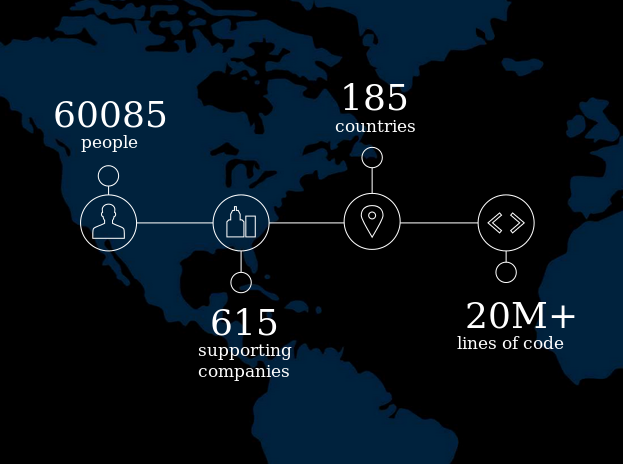
\includegraphics[width=.3\textwidth]{images/global_community.png}
      \caption{Dimensão da OpenStack Foundation\footnote{Imagem retirada de \url{http://www.openstack.org/}} em 05/09/2016}
    \end{figure}
    \item \textbf{Lista de emails:} \footnotesize{\url{http://lists.openstack.org/pipermail/foundation/}}
  \end{itemize}
}

\note[itemize]{
  \item Indivíduos têm direito a voto desde que estejam ativos
  \item Qual é o peso do voto de um indivíduo comparado a uma empresa?
  \item Indivíduos de empresa votam?
}

\frame{
  \frametitle{Comitê Técnico}
  \begin{columns}
    \begin{column}{.5\textwidth}
      \begin{figure}
        \centering
        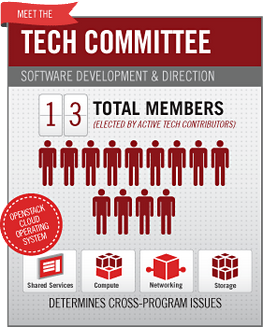
\includegraphics[width=.8\textwidth]{images/tech_comittee.png}
        \caption{Imagem retirada de \footnotesize{\url{http://www.openstack.org/foundation/}} em 05/09/2016}
      \end{figure}
    \end{column}
    \begin{column}{.5\textwidth}
      \begin{itemize}
        \item Rumo do projeto
        \item Decisões técnicas que afetem múltiplos componentes
      \end{itemize}
    \end{column}
  \end{columns}
}

\frame{
  \frametitle{Corpo de Diretores}

  \begin{columns}
    \begin{column}{.5\textwidth}
      \begin{figure}
        \centering
        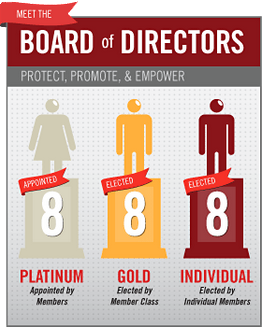
\includegraphics[width=.8\textwidth]{images/board.png}
        \caption{Imagem retirada de \footnotesize{\url{http://www.openstack.org/foundation/}} em 05/09/2016}
      \end{figure}
    \end{column}
    \begin{column}{.5\textwidth}
      \begin{itemize}
        \item Estratégica
        \item Financeira
        \item \textbf{Lista de emails:} \footnotesize{\url{http://lists.openstack.org/pipermail/foundation-board/}}
      \end{itemize}
    \end{column}
  \end{columns}
}

\note[itemize]{
  \item Lista de emails para formulação de atas e anúncio de programação de summits
}

\frame{
  \frametitle{Comitê de Usuários}

  \begin{columns}
    \begin{column}{.5\textwidth}
      \begin{figure}
        \centering
        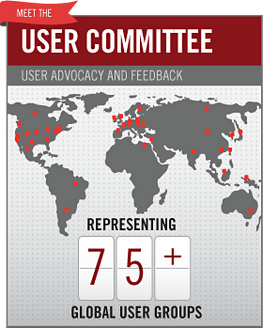
\includegraphics[width=.8\textwidth]{images/user_comittee.png}
        \caption{Imagem retirada de \footnotesize{\url{http://www.openstack.org/foundation/}} em 05/09/2016}
      \end{figure}
    \end{column}
    \begin{column}{.5\textwidth}
      Criado recentemente para dar representatividade aos grupos globais perante o corpo diretivo e comitê técnico.
    \end{column}
  \end{columns}
}

\frame{
  \frametitle{Outros}
  Não são listados na página oficial mas possuem lista de emails ativa:

  \begin{itemize}
    \item Defcore Committee
      \begin{itemize}
        \item Padronização de ``todos os produtos \textit{OpenStack}''
        \item \textbf{Página:} \footnotesize{\url{https://wiki.openstack.org/wiki/Governance/DefCoreCommittee}}\footnote{Visitado em 09/09/2016}
        \item \textbf{Lista de emails:} \footnotesize{\url{http://lists.openstack.org/pipermail/defcore-committee/}}
      \end{itemize}
  \end{itemize}
}
